\documentclass[preprint]{aastex} 

\usepackage[top=1in, bottom=1in, left=1in, right=1in]{geometry}
\usepackage{amsmath}
\usepackage{graphicx}
\usepackage{mdwlist}
\usepackage{natbib}
\usepackage{natbibspacing}
\setlength{\bibspacing}{0pt}
\setlength{\parskip}{0pt}
\setlength{\parsep}{0pt}
\setlength{\headsep}{0pt}  
\setlength{\topskip}{0pt}
\setlength{\topmargin}{0pt}
\setlength{\topsep}{0pt}
\setlength{\partopsep}{0pt}
\setlength{\footnotesep}{8pt}
\pagestyle{empty}
\citestyle{aa}

\def\kperp{k_{\bot}}
\def\kpar{k_{\|}}
\def\k{{\bf k}}
\def\sky{{\theta}}
\def\HI{{H{\small I }}}
\def\HII{{H{\small II }}}
\def\xHI{{x_{\rm\HI}}}

%\usepackage{subfig}
%\usepackage[countmax]{subfloat}

%Project Description (8-pages maximum), including the following:
%- A statement of which of the four categories of MSIP is most appropriate
%for this proposal as the first sentence (see section II. Program Description).
%- A scientific justification. For Open Access Capabilities, explain the
%uniqueness and lack of general availability of the capability.
%- A description of the broader impacts, including student training.
%- A description of benefits to the community (observing time, data products, etc.)
%- An outline of the project management plan (where appropriate).
%Note: Results from Prior NSF Support should not be included. Links to URLs may
%not be used.
\begin{document}
%\title{Hydrogen Epoch of Reionization Array}
\title{HERA: Illuminating Our Early Universe\\
{\it For the Mid-Scale Science Projects category of the Mid-Scale Innovations Program}} 

% A statement of which of the four categories of MSIP is most appropriate
%for this proposal as the first sentence (see section II. Program Description).

%This proposal targets the Mid-Scale Science Projects category of the Mid-Scale Innovations Program solicitation. The Hydrogen Epoch of Reionization Arrays (HERA) is a program for using the unique capabilities of the 21~cm hyperfine line to trace neutral hydrogen through the cosmic dawn of our Universe.  The HERA roadmap that was submitted to the {\it New Worlds, New Horizons of Astronomy and Astrophysics} 2010 decadal survey, (hereafter NWNH) was given ``top priority in this [Radio, Millimeter, and Sub-millimeter] category of recommended new facilities for mid-scale funding." The HERA roadmap proceeded in three stages: HERA-IB called for \$25M to complete the PAPER and MWA experiments; HERA-II budgeted \$62M for an array with 0.1 km$^2$ of collecting area capable of characterizing the power spectrum of cosmic reionization in detail; HERA-III targeted 1 km$^2$ of collecting area to image reionization structures in detail.

% XXX mcquinn: highlight a couple of key sentences?
{ \setlength{\parindent}{0cm}
The Hydrogen Epoch of Reionization Arrays (HERA) roadmap is a staged 
program that uses the unique properties of the 21~cm line from neutral 
hydrogren to probe the 
<<<<<<< HEAD
Epoch of Reionization (EoR) and the preceding Dark Ages.  These epochs
correspond to
when the first stars and black holes heat and reionize the
Universe following cosmic recombination, roughly
0.3~Gyr to 1~Gyr after the Big Bang. Direct observation of the evolution of the
large scale structure of reionization via the \HI 21~cm line will have a profound impact on our
understanding of the birth of the first galaxies and black holes, their
influence on the intergalactic medium (IGM), and cosmology.}  

HERA was ranked the ``top priority in the Radio, Millimeter, and Sub-millimeter
category of recommended new facilities for mid-scale funding" as part of the
{\it New Worlds, New Horizons of Astronomy and Astrophysics} decadal survey
(\citealt{astro2010}; hereafter NWNH).  
The HERA roadmap envisioned a series of
radio interferometers constructed throughout the decade, starting with the current
Donald C. Backer Precision Array to Probe the Epoch of Reionization (PAPER) and 
the Murchison Widefield Array (MWA) instruments 
aimed at characterizing
foregrounds and laying the groundwork for detecting the EoR power
spectrum. A second-generation HERA instrument would measure the EoR power spectrum in
detail and reveal how early structure in the Universe formed, and a
third-generation instrument would image the EoR with high SNR. 

% XXX would like to highlight the PAPER result here
Using the advances spearheaded by
PAPER and the MWA,
we propose to build the next generation of HERA in stages of 127, 331, and 568 elements,
observing in the 50--225MHz band.
Each stage of HERA is scoped to deliver new science capabilities that advance our
understanding of reionization in a timely manner.
\begin{itemize}\setlength{\parskip}{0pt}\itemsep0pt
\item HERA~127 will measure the rise and fall of the EoR power
spectrum, constraining the timing and duration of reionization.
\item HERA~331 will measure the shape of the power spectrum over
a significant range in wavenumber, determining the features and distribution of
the first galaxies that dominate cosmic reionization.
\item HERA~568 will extend precision power-spectrum observations
into the Dark Ages and start direct imaging of the IGM during reionization.
\end{itemize}
{ \setlength{\parindent}{0cm}
Taken together, this program
not only fulfills the NWNH goal of detailed power spectrum
characterization as a second-generation EoR experiment, but is also
capable of imaging the EoR---a task previously considered possible only for
third-generation instruments.}
%Further, given recent advances in our understanding, these goals may be 
%undertaking at a substantially lower budget than contained in the earlier roadmap.}

\vspace{-0.25in}
\section{Scientific Justification}
\label{SJsec}

The last unexplored phase in the evolution of luminous structures in the
Universe begins with the birth of the first stars and culminates with the full
ionization of the IGM $\sim$500 Myrs later.  During the Dark Ages
(z$\ge$15) and the Epoch of Reionization (z$\sim$15--6), a wealth of
astrophysical and cosmological phenomena are at work.  The precise properties
of the IGM depend on the nature and distribution of the first luminous sources
(eg. typical masses, UV escape fractions, biased structure formation), the
efficiency and abundance of heating sources (eg.  X-ray binaries, shocks, or
even dark matter annihilations), the formation of the first supermassive black
holes, and the relative velocity of baryonic matter and dark-matter halos,
among other effects.  Exploration of the Dark Ages and EoR and the evolution of
the IGM during these epochs has been heralded as one of the top three
``priority science objectives chosen by the [NWNH] survey committee for the
decade 2012-2021."

Thus far, a number of indirect probes have been used to understand cosmic
reionization.  These include observations of Gunn-Peterson attenuation by the
IGM toward the most distant quasars \citep{fan_et_al2006},
kinetic Sunyaev-Zel'dovich anisotropies in the CMB temperature \citep{zahn_et_al2012_trunc}, CMB
polarization \citep{page_et_al2007,planck_et_al2013}, and the
demographics of Ly$\alpha$ emitting galaxies
\citep{treu_et_al2013}, as summarized in Figure~\ref{fig:x_i_Xray}a.  Unfortunately,
these ground-breaking results have limited reach: the
Gunn-Peterson effect and related phenomena saturate at low neutral fractions,
and the CMB provides only an integral measure of %the optical depth
the EoR looking % XXX check with McQuinn if this phrasing works
back to recombination.  Moreover, many of these indirect observations are in
tension with one another, underscoring both the difficulty in interpreting
these results, and the fact that reionization was a complex process.


\begin{figure}[t]\centering
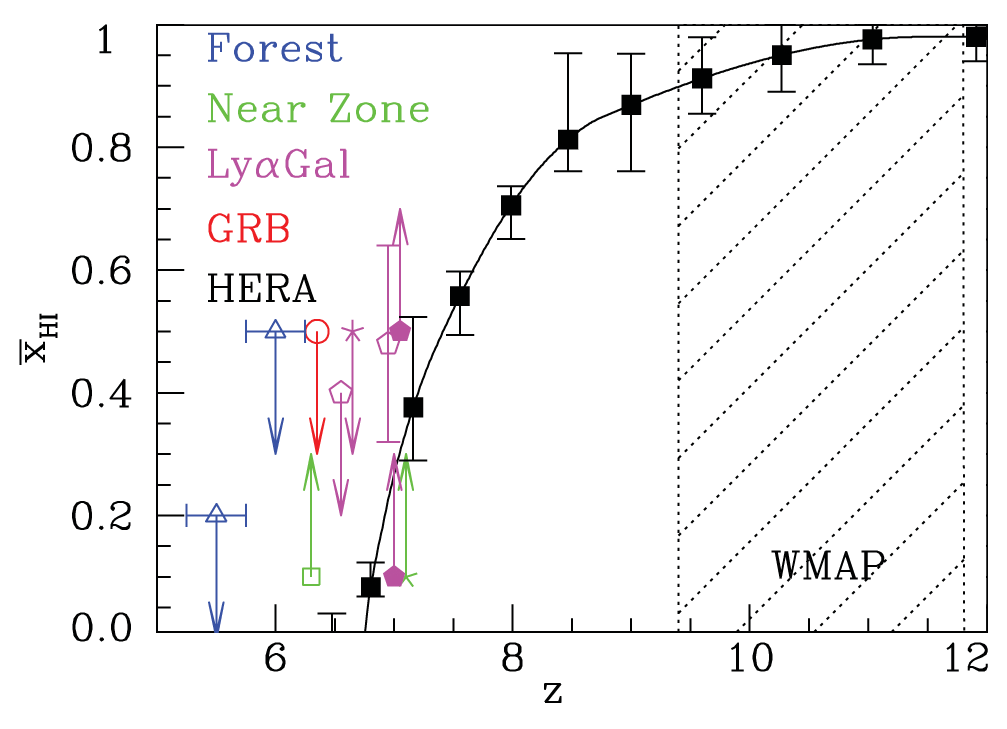
\includegraphics[height=2.25in]{plots/constraints_crop.pdf}  % XXX choose crop vs regular
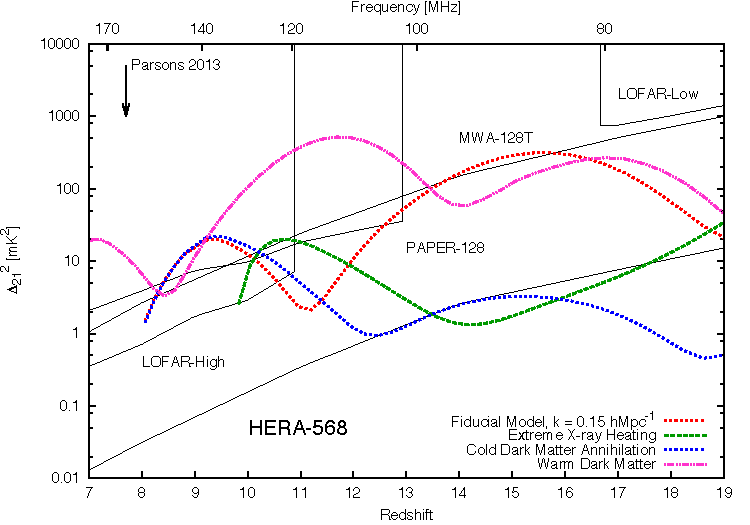
\includegraphics[height=2.25in]{plots/Xray.pdf} 
\caption{\small 
Left: Adapted from \citet{robertson_2013}, this figure shows existing
constraints on $\xHI$ during reionization (colored symbols), along with a
reionization history consistent with these measurements (black line). The
constraints HERA would provide are indicated with black markers (with the constraint
that $\xHI$ steadily decreases over this redshift range). At redshifts 8--12
21~cm emission may be the only precision probe of the neutral fraction.  
Right: HERA’s substantial sensitivity at low frequencies opens a window to
pre-reionization physics. Shown here are power spectrum amplitudes (at $k =
0.15h$~Mpc$^{-1}$) as a function of redshift for various IGM heating models,
along with predicted sensitivities.
}\label{fig:x_i_Xray} \end{figure}

The 21~cm hyperfine transition has been recognized as potentially the most
powerful probe of the evolution of the IGM during cosmic reionization, and into
the preceding Dark Ages \citep{morales_wyithe2010,furlanetto_et_al2006}.
%
The study of the three-dimensional
evolution of large scale structure in the IGM via the \HI 21~cm line has the
potential to become `the richest of all cosmological data sets', and is expected
to have a science impact comparable to that of the CMB
\citep{barkana_loeb2005a,loeb_zaldarriaga2004}).  As emphasized in
NWNH: ``The panel concluded that to explore the discovery
area of the epoch of reionization, it is most important to develop new
capabilities to observe redshifted 21~cm \HI emission, building on the legacy of
current projects and increasing sensitivity and spatial resolution to
characterize the topology of the gas at reionization."  
%Although early 21~cm EoR experiments with limited sensitivity are targeting statistical detections
%of the power spectrum of reionization, the 21~cm signal versus redshift can
%eventually be reconstructed into three-dimensional maps of the evolution of
%cosmic structure that would greatly improve our understanding of the
%cosmological and astrophysical evolution of the universe
%\citep{furlanetto_et_al2006,mao_et_al2008,morales_wyithe2010}. 
As a high
sensitivity instrument with broad frequency coverage, HERA will be capable of
painting a consistent and uninterrupted picture of not just the EoR, but also
into the preceding Dark Ages.  
% XXX Miguel will tie this into figures.

% XXX is there text from this paragraph to save?
%The new window into high-redshift 21~cm observations provided by HERA
%will begin to explore the rate and density of massive black holes formed in the
%early universe \citep{pritchard_loeb2010} via their X-ray emission (see Figure \ref{fig:Xray}), 
%how velocity streaming between baryonic 
%matter and the dark matter halos affected early structure formation and the onset
%of Ly$\alpha$ emission \citep{visbal_et_al2012}, and will lay the groundwork for future
%efforts to explore how 
%cosmological models can be improved via measurements of redshift-space distortions,
%artificial anisotropies introduced via the Alcock-Paczy\'inski effect, and
%gravitational lensing signals\citep{furlanetto_et_al2006}.
%As illustrated in Figure \ref{fig:x_i}, observing the 21~cm line 
%through this epoch with HERA-568 
%promises to determine the ionization history of our universe much more precisely,
%and at higher neutral fractions, than is possible with other existing techniques.  These measurements can
%be used to move beyond characterizing the timing and duration of reionization to
%explore which galaxies dominate the integrated UV luminosity density, what the escape fraction
%of UV photons is in early galaxies, and how feedback from early star formation affects low-mass galaxies and the integrated global %ionization profile versus
%redshift.  Moreover, measurements of the slope of the power spectrum of 21~cm emission through
%reionization (Figure \ref{fig:FourPanContour}) determine the size of ionization bubbles for at
%various stages of reionization, which
%constrains the relative contributions to the ionizing background of halos as a function of mass,
%and helps us understand how efficiently early structures cooled and formed stars.

%The evolution of the \HI 21~cm signal from the neutral IGM depends on miriad
%physical processes, including: general large scale structure evolution, IGM
%ionization by the first galaxies and black holes, and the complex interplay
%between the gas kinetic and excitation temperatures, and the temperature of the
%CMB \citep{furlanetto_et_al2006}. The gas kinetic temperature can be affected
%by shocks or pervasive X-rays from the first luminous sources, and the \HI
%excitation temperature can be dictated by collisions, CMB photons, or resonant
%scattering of ambient Ly$\alpha$ photons, depending on epoch
%\citep{pritchard_loeb2012}.  The relative importance of these competing effects
%is sensitive to, among other things, the expansion of the universe, the
%ignition of the first stars and galaxies, the formation of the first massive
%black holes \citep{mesinger_et_al2013}, and the relative velocity of baryonic
%matter and dark-matter halos \citep{mcquinn_oleary2012}.  

In the past decade, considerable effort has gone into modeling the complex astrophysics
of reionization
% XXX if more cites, add Shull, Haiman, Furlanetto, Oh, Gnedin, Shaver
\citep{santos_et_al2010,mesinger_et_al2011,wyithe_loeb2004}. However, bridging the
enormous scale difference between the self-shielding regions that are the
primary sinks of ionizing photons and volumes required for statistically
representative samples of cosmic structures remains an open problem. 
% XXX cite Choudhury, Haehnel, Regan 2009
Basic constraints on theoretical models remain rudimentary, and the most
fundamental questions concerning the process of reionization remain open. 
When did
reionization occur, and over what timescale?  What objects dominated the
radiation field? how were the objects distributed? Did the first generation of
stars enhance or suppress the formation of subsequent stars in the original
halo and smaller nearby halos? Without measurements such as those made possible by HERA,
further progress on understanding first galaxy formation and
cosmic reionization remains problematic. 

\begin{figure}[t]\centering
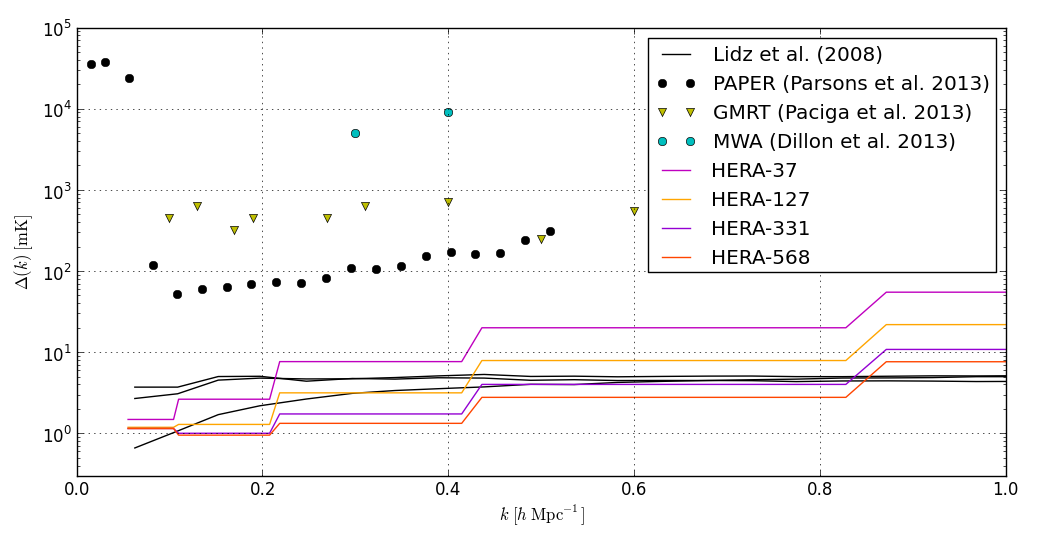
\includegraphics[height=2.40 in]{plots/eor_pspec.png}
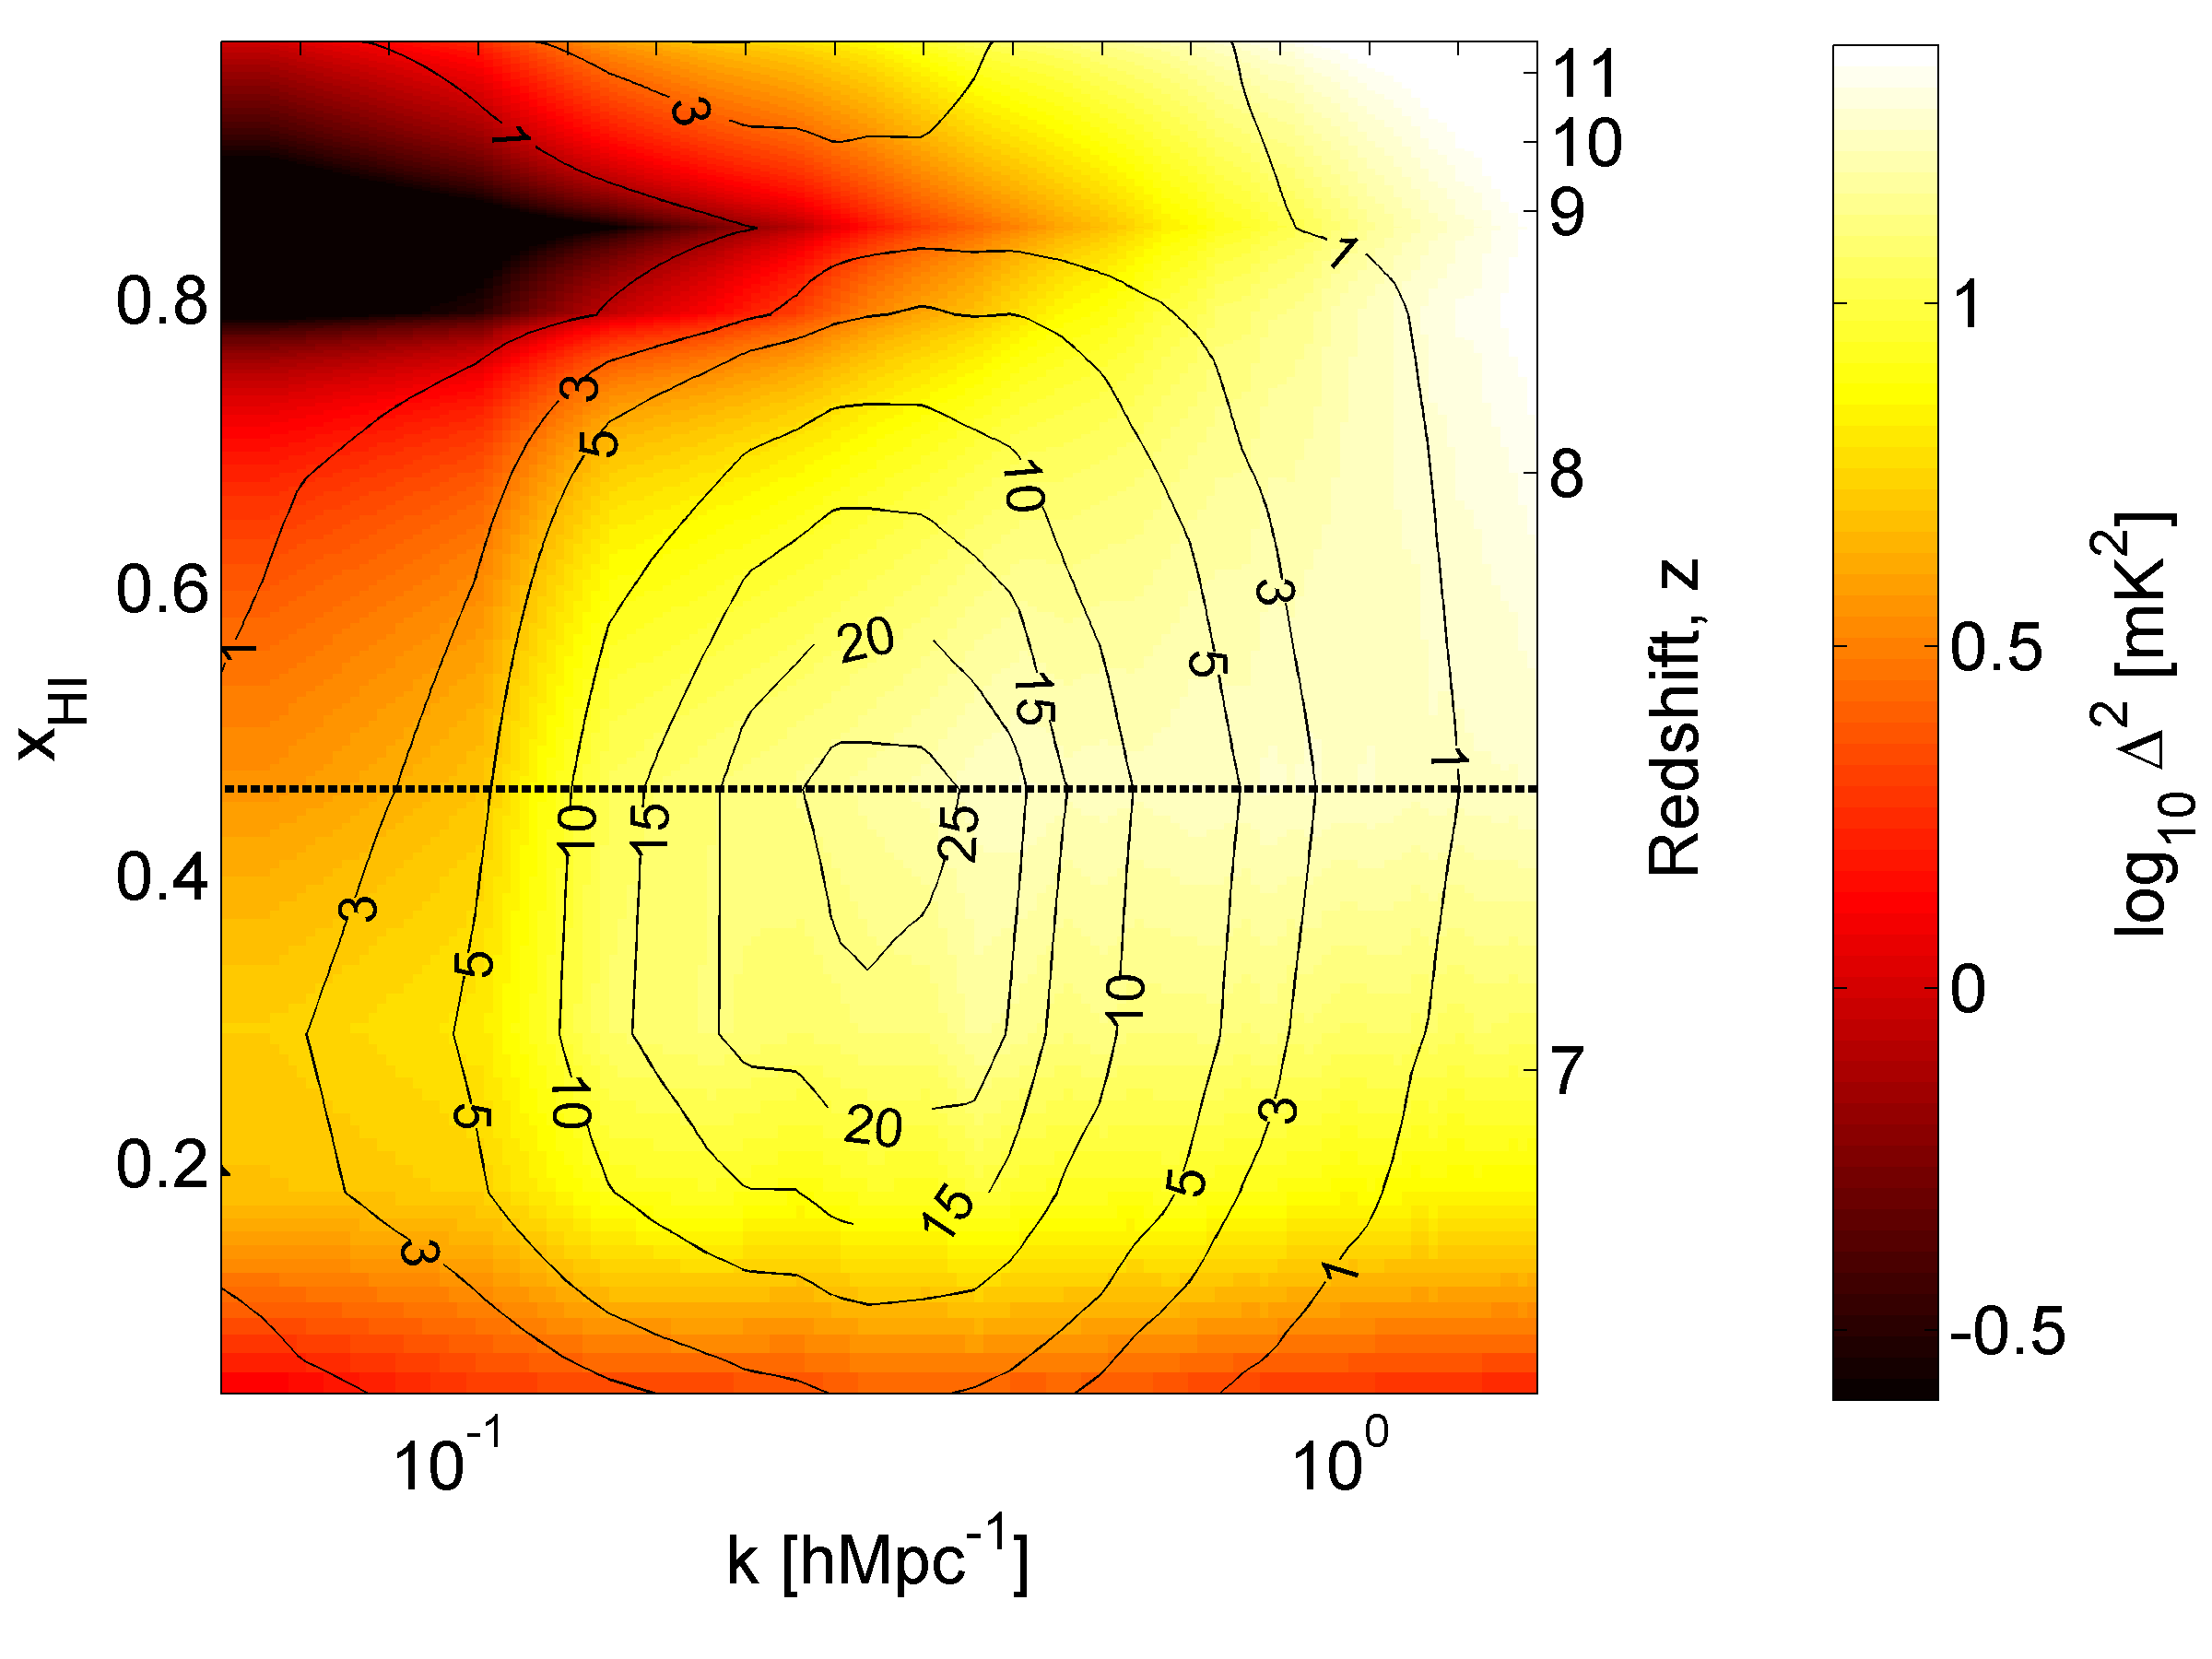
\includegraphics[height=2.45 in]{plots/hera_snr_contour.png} % XXX awaiting latest from Judd
\caption{\small 
Left: Power-spectrum sensitivities for three stages of
HERA (solid) relative to a fiducial ionization model (dashed line at $\xHI=0.47$ in both panels).  
In addition
to a staged array size, sensitivity curves reflect
a staged improvement in analysis software that expands the range
of modes that are not corrupted by systematics. 
Right: The color surface shows the rise and fall of the 21~cm power spectrum from 
\citealt{lidz_et_al2008} as a function of neutral fraction $\xHI$ (and hence redshift).
The spectrum initially follows the dark matter fluctuations at the upper edge
of the plot, falls as the densest regions reionize at $\xHI=0.8$, rises and flattens as galaxies ionize large bubbles in the IGM
($0.6<\xHI<0.2$), and finally
falls again as reionization completes at the bottom of the
plot. Contours indicate the predicted signal-to-noise ratio of HERA~568 observations
throughout reionization.
}\label{fig:eor_pspec} 
\end{figure}

% XXX from mesinger
%you don't mention the pre-reionization signal.  HERA could be transformative in
%reaching beyond the late stages of reionization, and seeing the imprint of the
%very first galaxies in the Lya and X-ray backgrounds.  This is really
%remarkable for 21cm, as these galaxies will be inaccessible through other means
%(with the exception of poor, integral constraints from the CMB).  The same
%cannot be said for the EoR.  Perhaps it is more appropriate for the
%later/longer proposal, but i would be nice to briefly stress that the
%sensitivity of the 21cm line to the IGM temperature means that we can study
%processes which heat the IGM.  These are likely dominated by X-rays from black
%hole binaries, but could have a strong, easily-identified contribution from
%Dark Matter annihilation in some models.  Additionally, the early redshifts
%corresponding to the Cosmic Dawn are great testbeds for popular LCDM
%alternatives, such as Warm Dark Matter, as the Universe is expected to be empty
%in these models.  This makes the 21cm signal during the pre-reionization Cosmic
%Dawn epoch a powerful probe of both astrophysics and cosmology.  Eventually,
%for the longer proposal, I can make the contour plots for HERA which are
%analogous to the ones in my paper with Aaron E-W.


\vspace{-0.25in}
\section{Foregrounds \& Lessons Learned from PAPER and MWA}
\label{LessonsSec}

The key challenge of 21~cm cosmology is isolating the faint EoR signal from
astrophysical foregrounds that are $\sim$5 orders of magnitude brighter. These foregrounds
are shown in recent MWA image 
in the left-hand panel of Figure \ref{fig:twoFGViews}. A major breakthrough in
21~cm cosmology---what enables us to propose HERA now---is the discovery of the
EoR Window.
% XXX gotta play up PAPER result here

21~cm cosmology observations and foreground isolation are best understood in
the three dimensional wavenumber space $\k$.  Because the \HI emission is a
narrow spectral line, the observed frequency of the emission can be mapped to
redshift or line-of-sight distance to provide an observed volume $\{x,y,z\}$ in
co-moving Mpc. This observed volume is Fourier transformed into a three dimensional
wavenumber cube $\{k_{x}, k_{y}, k_{z}\}$. For graphical simplicity, the angular
wavenumbers are typically averaged ($\{k_{x},k_{y}\}\rightarrow\kperp$) to
produce line-of-sight wavenumber $\kpar$ vs.\ angular $\kperp$. 
%Interferometric measurements are of the angular Fourier modes in many
%frequency channels (visibilities), so in the absence of widefield effects only
%a Fourier transform in the frequency direction and a coordinate mapping is
%needed to obtain the 3D $\{k_{x}, k_{y}, k_{z}\}$ measurements
%\citep{morales_hewitt2004}.) 
The anticipated mean spatial isotropy of the signal allows measurements within the 3D wavenumber space to be
squared and averaged in shells to produce the spherical power spectrum
presented in Figure \ref{fig:eor_pspec}.

A significant recent advance in 21~cm cosmology has been understanding how smooth-spectrum
foreground emission interacts with the instrument to produce the EoR Window.
Through a concerted theoretical and observational campaign
\citep{morales_et_al2012,parsons_et_al2012b,vedantham_2012,Datta_2010,hazelton_et_al2013,pober_et_al2013,parsons_et_al2013,dillon_et_al2013b_trunc}
we now understand that the foreground contamination is confined to a `wedge' in
$\kpar$ vs.\ $\kperp$, as demonstrated by the PAPER observations in the
righthand panel of of Figure \ref{fig:twoFGViews}. This wedge is the result of
the smooth spectrum foregrounds (low $\kpar$) interacting with the inherent
chromaticity of an interferometer. Deep imaging similarly suppresses the 
contributions from polarized foregrounds \citep{bernardi_2013_trunc,moore_et_al2013}. 
This leaves the region above the wedge isolated from the
foreground emission---a window through which we can observe the EoR.


Observations with PAPER and the MWA have now confirmed the presence of the EoR Window
\citep{pober_et_al2013,dillon_et_al2013b_trunc}, including suppression by more than 4
% XXX mcquinn: awkward phrasing
orders-of-magnitude (8 in mK$^{2}$) to the thermal noise floor of current
PAPER observations \citep{parsons_et_al2013}. This is a major advance---we can
suppress foregrounds and we understand the instrumental and analysis
characteristics needed to perform the EoR measurement. The MWA and PAPER teams
have been at the forefront of developing the EoR Window, writing all of the % XXX is "all" going to make people cranky?
papers in the literature and developing the individual baseline
(delay-spectrum) and full power spectrum (imaging) analyses to exploit this
insight. 

% XXX principles of building this knowledge into instrument design

\begin{figure}[t] \centering
%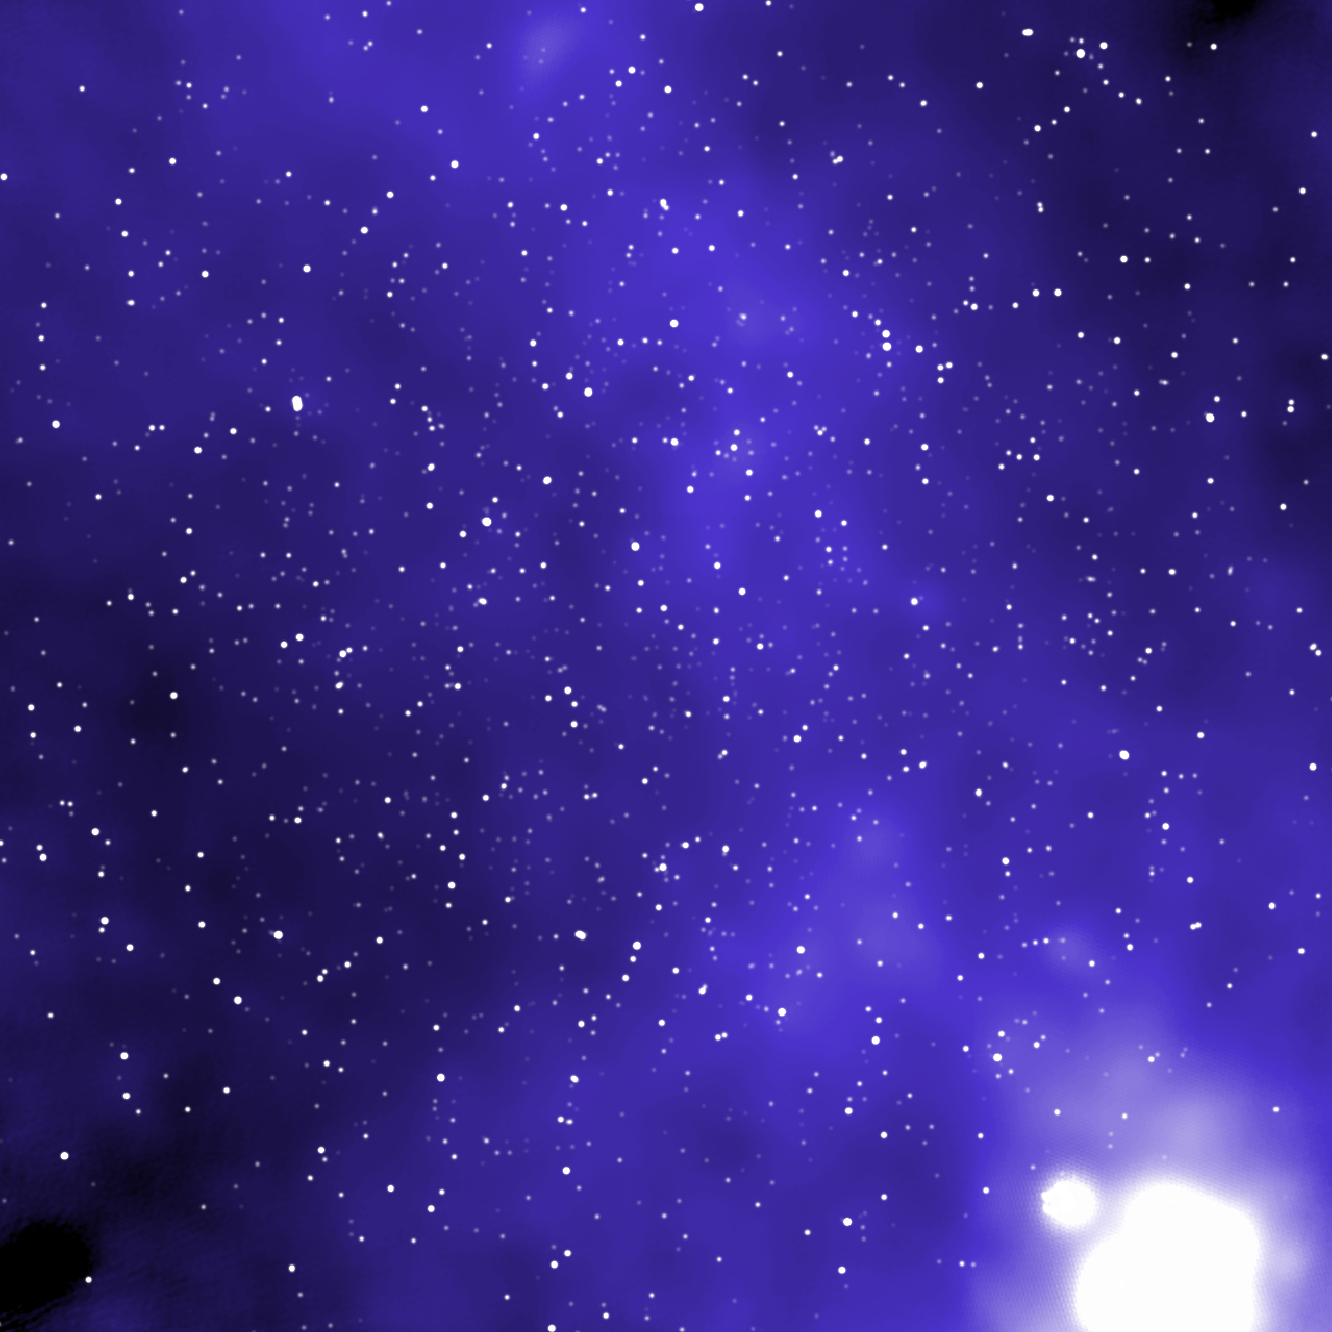
\includegraphics[width=6.5in]{plots/MWApretty.png} 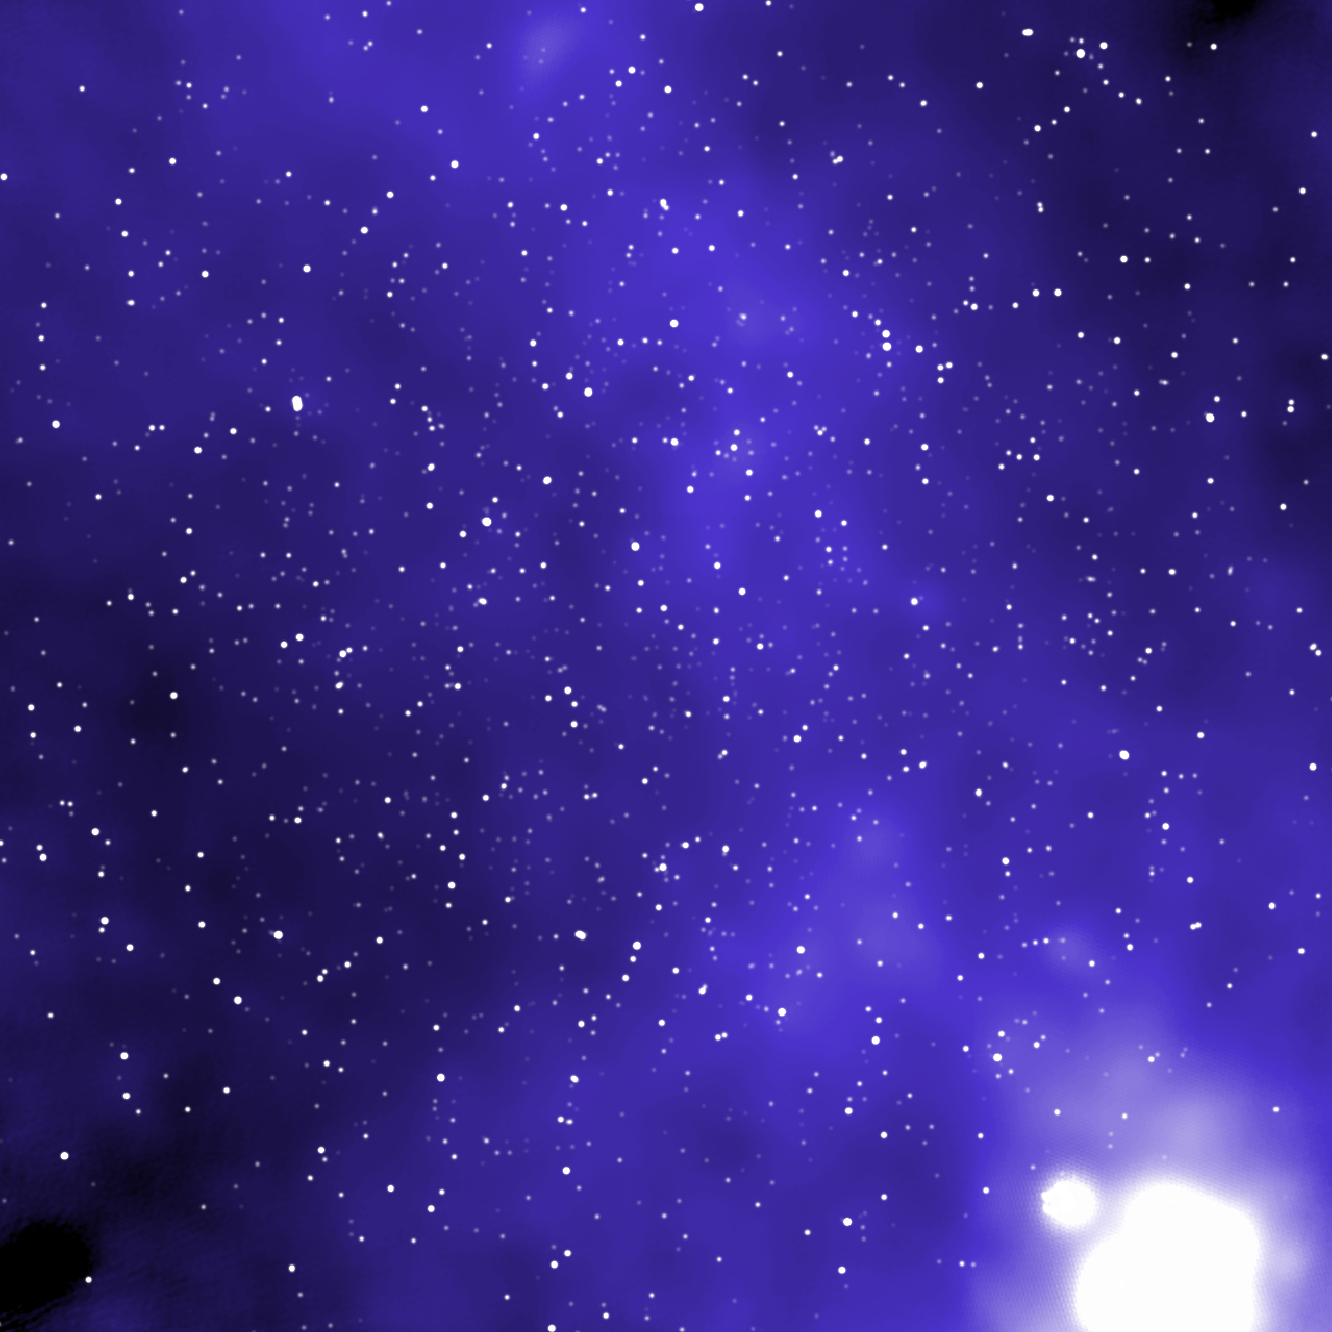
\includegraphics[width=3.6
%in]{plots/MWApretty.png}
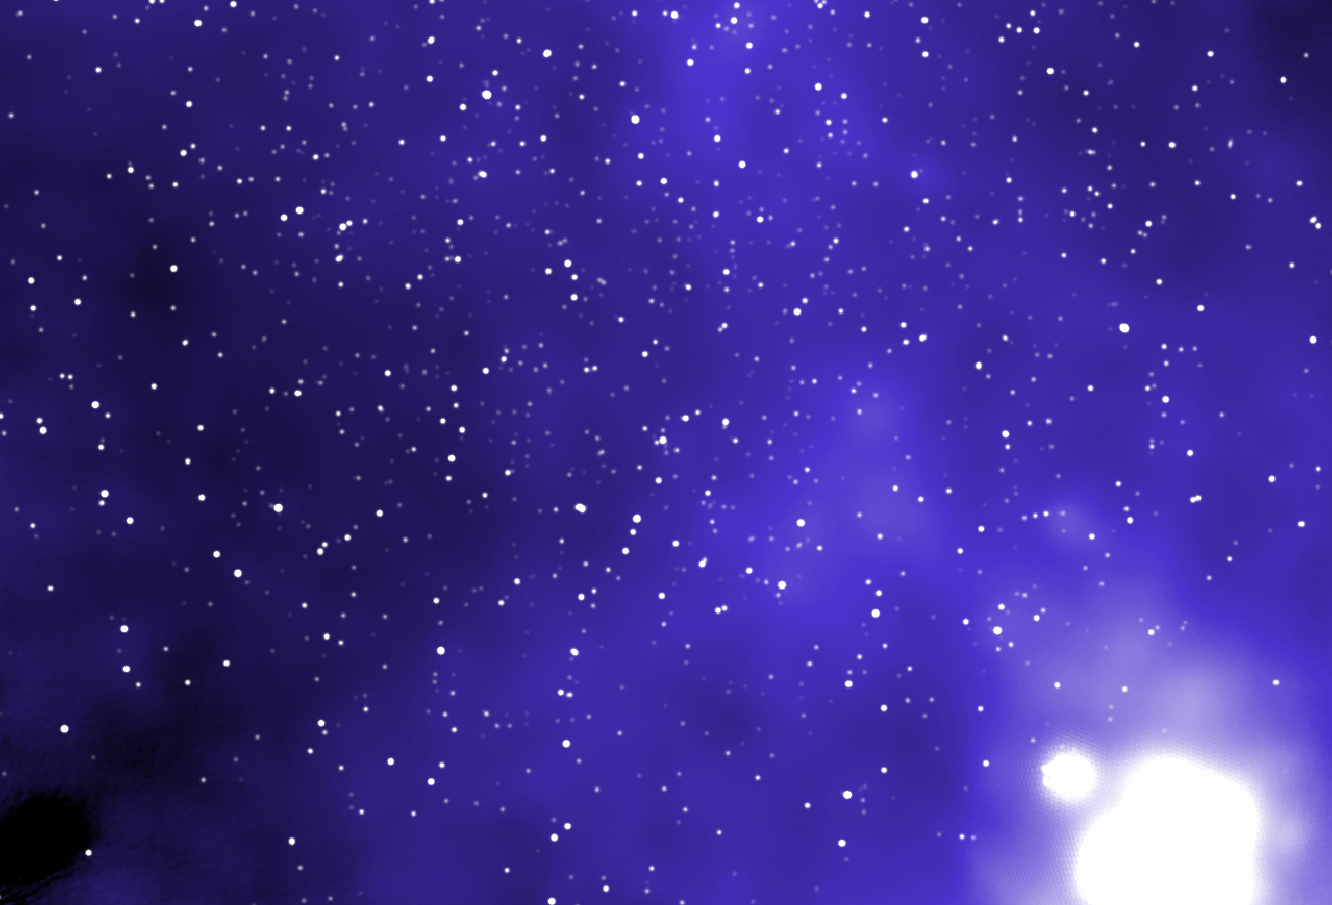
\includegraphics[height=2.5in]{plots/MWApretty_crop.png} 
~ %gutter btwn graphics
%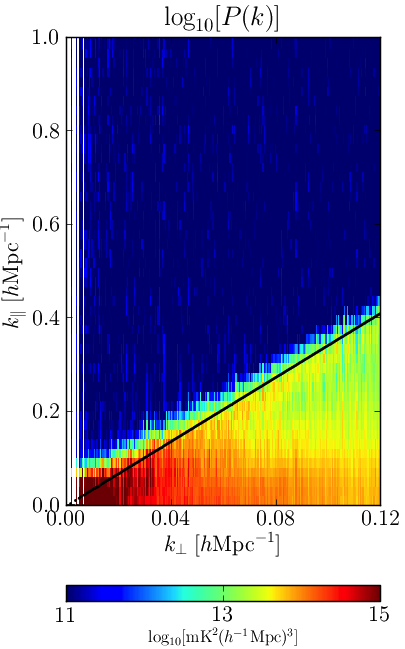
\includegraphics[width=2.4 in]{plots/wedge_tall.png}
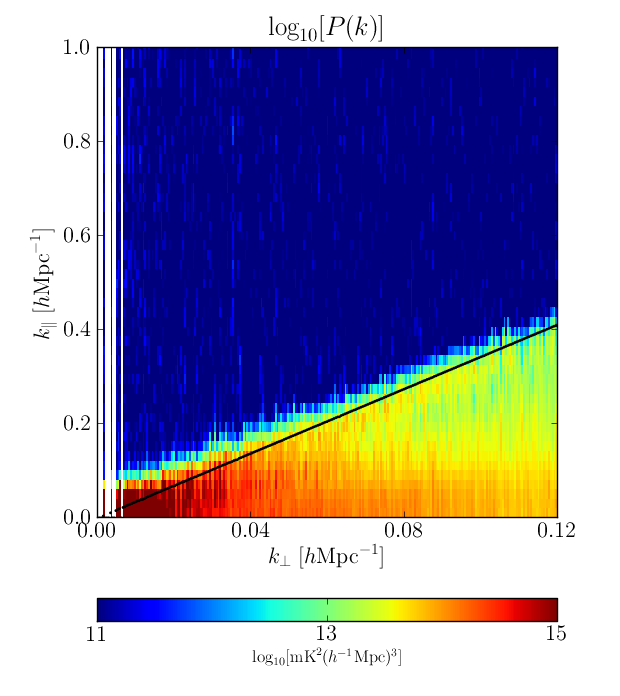
\includegraphics[height=2.5in]{plots/wedge_tall_wide.png} \caption{\small Left:
Foregrounds imaged on the MWA using FHD software developed by Morales' group
\citep{sullivan_et_al2012_trunc}.  This image, which spans $\sim$$30^{\circ}$ and
includes both point-source and diffuse emission (with the Vela and Puppis SNRs visible in the
bottom-right), illustrates the power of imaging methods for reducing
polarization leakage and foreground systematics.  
Right: Foreground contamination in line-of-sight $\kpar$ vs.\ angular $\kperp$
as observed using PAPER \citep{pober_et_al2013}, with
the analytic prediction of the horizon limit to foreground emission (solid black).
Bright foreground emission is
confined to a wedge (lower right) as predicted by
\citep{morales_et_al2012,parsons_et_al2012b,vedantham_2012,Datta_2010}, falling
by orders-of-magnitude to below the thermal noise in the EoR Window (blue
region). This insight has lead to sensitivity-limited upper limits and the
first meaningful constraints on EoR via 21~cm emission in
\citet{parsons_et_al2013}.
}\label{fig:twoFGViews} \end{figure}

\vspace{-0.25in}
\section{HERA}
\label{PDsec}
\begin{figure}[t]\centering
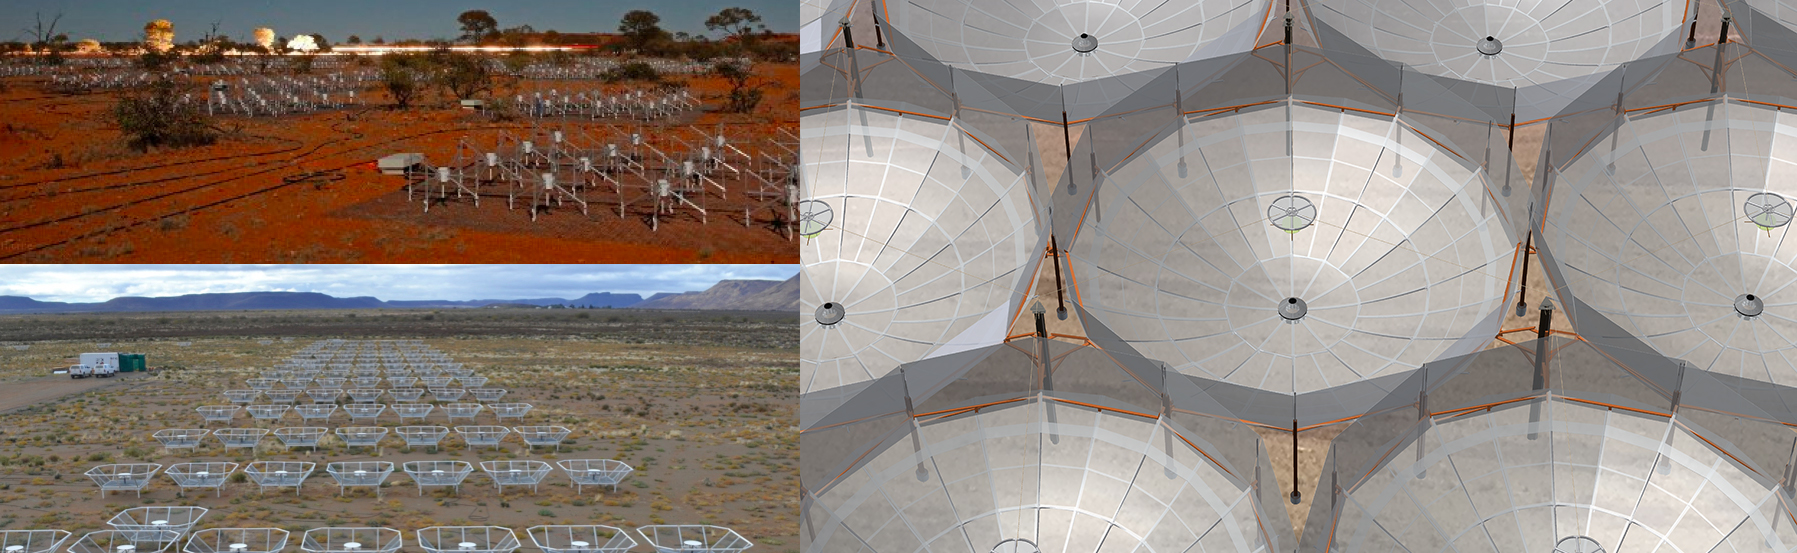
\includegraphics[width=6.5in]{plots/PAPER_and_MWA_and_HERA.jpg}
\caption{\small
The MWA (top left) and PAPER (bottom right) arrays, each currently deployed with 128 elements.
The 14-m HERA element (right) dramatically improves sensitivity
while delivering the spectral smoothness and stability of response that
are required for managing foregrounds.
The core of HERA~568 consists of a redundant hexagonal array with
outrigger antennas (not shown) for imaging and foreground mitigation.
}
\label{HERAfig}
\end{figure}

HERA will be built in stages at the Karoo Radio Observatory reserve in South Africa near the
current PAPER deployment, up to a final size of 568 antenna elements.
HERA 
incorporates numerous lessons learned from first-generation 21~cm EoR experiments.
It features a 14-m zenith-pointing dish optimized for sensitivity and foreground suppression,
a dense hexagonal core to facilitate redundant baseline calibration and
delay-spectrum analysis (see Figure \ref{HERAfig}), and a distribution of outrigger antennas to provide
complete uv coverage to $\sim$700~m for foreground imaging and mitigation.
HERA draws on the technical heritage of the MWA, PAPER,
EDGES and MITEoR. Specific examples include the antenna feed and correlator of
PAPER, receiver node and field digitization from the MWA, absolute radiometric
calibration from EDGES, redundant baseline calibration from MITEoR \citep{zheng_et_al2013_trunc}, the
delay-spectrum analysis from PAPER, and the precision imaging and foreground
removal software from the MWA.

%Incorporated into the design of HERA are new aspects that reflect our current understanding of the optimal balance between sensitivity and foreground systematics.  

The HERA antenna is an example of this technical heritage. The spectral
smoothness and the stability of the antenna response determine the precision to
which astrophysical foreground emission can be separated from the cosmological
21~cm emission. HERA uses the PAPER dipole feed---modified slightly for wider
bandwidth---suspended over a 14-m parabolic dish (Figure \ref{HERAfig}). The
short ($\sim$5~m) focal height of the dishes is central to limiting the path
length of reflections, whose time-delay gives rise to chromatic antenna
sensitivity. The zenith pointing enhances the stability of the antenna response
(as found for PAPER), short cables to in-field digitizers limit the length of cable
reflections (MWA), and absolute calibration (EDGES) are all designed to provide
an extremely stable and smooth spectral response. Similarly the antenna layout
uses the dense core, outriggers, and symmetric configuration of the MWA,
combined with redundant baselines within the core that improve sensitivity
and enable a new mode for calibration (PAPER, MITEoR). Together
these advances enable HERA to have the science reach envisioned in the decadal
survey while fitting within the MSIP funding envelope.

HERA follows a staged deployment in both physical construction and scientific processing.  In
each deployment stage, improvements are incorporated into the system and new
science capabilities are unlocked.  This approach has the advantage of both
providing early access to science and reducing the project risk by testing systems
early and changing them incrementally.  As shown in Figure \ref{fig:eor_pspec}, each
stage of HERA brings an associated improvement in sensitivity that allows key
aspects of 21~cm reionization science to be addressed.  The timeline of HERA
development, along with the associated science products, is outlined below. 

\noindent{\bf Year 1--Infrastructure and First 37 Antennas (FY 2015)}.  
\begin{itemize}\setlength{\parskip}{0pt}\itemsep0pt
\vspace{-7pt}
  \item Install infrastructure $\sim$10~km from the current PAPER site at the Karoo Radio Observatory in South Africa. Includes ground leveling, power and basic network connectivity.
  \item Move existing PAPER-128 antennas, correlator, and EMC container to new site.
  \item Install first 37 HERA antennas and instrument with existing PAPER feeds and electronics. 
  \item Begin development of improved HERA baluns, receivers, feeds, and 
nodes using the PAPER and MWA technical heritage \citep{bradley_et_al2005,lonsdale_et_al2009_trunc,tingay_et_al2013_trunc} 
and the in-situ antenna calibration system based 
on EDGES \citep{rogers_2012}. Continue development of delay-spectrum \citep{parsons_et_al2012b}, 
Fast Holographic Deconvolution (FHD; \citealt{sullivan_et_al2012_trunc}) and 
optimal estimator software \citep{dillon_et_al2013b_trunc}.
\end{itemize}


\noindent{\bf Year 2--Hardware Commissioning and Deep Foreground Survey (FY 2016)}.  
\begin{itemize}\setlength{\parskip}{0pt}\itemsep0pt
\vspace{-7pt}
  \item Commissioning observations using a hybrid array of 37 HERA antennas in a close-packed hexagon surrounded by 91 PAPER antennas in an imaging configuration.
  \item Perform a polarized foreground survey using hybrid-antenna capability of FHD. Determine on-sky beam response of HERA antennas to facilitate future source subtraction efforts.
  \item Finalize site infrastructure (high-bandwidth optical network, surveying, trenching).
  \item On-antenna commissioning of new feeds, receivers, nodes, and calibration systems in Green Bank and South Africa.
  \item Build out to 127 HERA antennas starts.
\end{itemize}


\noindent{\bf Year 3--HERA 127 and Detecting the Rise and Fall of Reionization (FY 2017)}.
\begin{itemize}\setlength{\parskip}{0pt}\itemsep0pt
\vspace{-7pt}
  \item Complete construction of HERA~127. Begin science observations Oct.\ 2016, again using the PAPER correlator.
  \item Begin analysis of a dataset capable of constraining the timing and duration of reionization. 
Analysis focuses on proven techniques based on PAPER delay-spectrum analysis, explorating subtraction of bright 
and polarized foregrounds.
  \item Begin deployment of HERA~331. Install node electronics for all 331 elements, and a new 331-element, 
GPU-based correlator in the Karoo Array Processing Building (KAPB).
  \item  Install new data storage infrastructure in the KAPB.  
Upgrade the UPenn analysis cluster.
\end{itemize}

\noindent{\bf Year 4--HERA 331 and Measuring the Evolution of the First Galaxies (FY 2018)}.
\begin{itemize}\setlength{\parskip}{0pt}\itemsep0pt
\vspace{-7pt}
  \item Finish construction of HERA~331. Begin science observations Oct. 2017.
  \item Complete science observations with HERA~331 Apr. 2018. Begin analysis of data to
characterize the evolution of the power spectrum and determining properties of the first galaxies.
  \item Continue analysis software development, emphasizing imaging-based subtraction techniques for expanding the EoR window.
  \item Begin build out to 568 antennas begins, including outrigger antennas to facilitate imaging and better foreground removal.
  \item Complete pipelines for EoR processing of HERA~568.
\end{itemize}

\noindent{\bf Year 5--HERA 568, Imaging Reionization and Exploring the Dark Ages (FY 2019)}.
\begin{itemize}\setlength{\parskip}{0pt}\itemsep0pt
\vspace{-7pt}
  \item Finish construction of HERA~568. Begin science observations Oct. 2018.
  \item Analysis push to enable imaging of the largest structures and extracting the full sensitivity of 
the instrument, including partially coherent baselines. 
\end{itemize}

\noindent
{\it The staged buildout of HERA enables cutting edge science at each stage while
mitigating risk by allowing the team to learn from experience along the way.}
HERA~127 will measure the rise and fall of the EoR power spectrum; HERA~331
will characterize the shape of the power spectrum and constrain the development
of the first galaxies; and HERA~568 will start to image reionization while
pushing power spectrum measurements into the Dark Ages.

% XXX check: was this stuff incorporated into a caption?
%In addition to pushing the sensitivity frontier, HERA will also extend the redshift frontier 
%to $z \sim 20$ and possibly beyond.  Measuring the power spectrum at higher, pre-reionization redshifts provides
%an incisive probe of astrophysical processes that are qualitatively different from those that
%drive reionization.  During the reionization era, the $21\,\textrm{cm}$ signal is driven by
%fluctuations in the ionization state of the IGM, while at higher redshifts the signal is determined
%by fluctuations in the spin temperature.  These fluctuations in turn depend sensitively on the nature of early heating sources  and their abundance, as well as on more exotic physics such as dark matter annihilation cross-sections.  Beginning with the midstages of its staged build-out, HERA will be in a unique position to probe the pre-reionization epoch that current-generation instruments are unable to reach (see Figure \ref{fig:x_i_Xray}).  With its ability to measure the power spectrum \emph{continuously} over an extremely large frequency range,
%HERA will also provide a longer lever arm for ionization history measurements than any other astronomical probe,
%as one can see in Figure \ref{fig:x_i_Xray}.
%
%{\sl Imaging reionization} In the later stages, HERA will become a powerful imaging instrument of cosmic reionization. Fiducial simulations of the expected \HI 21~cm signal on 25' scales predict regions with contrasts of about 10mK at 150MHz, or flux densities of up to 0.5 mJy/beam \citep{mcquinn_et_al2007}. The expected thermal noise for HERA 576 is 60 uJy, hence these regions could be detected at high confidence across redshifts $6<z<12$. Figure \ref{imaging} shows the predicted images of the \HI 21 structures  assuming the properties of HERA 547. The large scale structure is easily detected, and imaged, with the later stages of HERA. Of course, reaching these sensitivity levels relies critically on foreground synchrotron removal. We will be exploring foreground removal techniques throughout the program, and in particular, in the latter stages. The resulting \HI 21~cm images will provide a key reference for imaging of the large scale galaxy distribution (the sources of reionization), using CO or [CII] intensity mapping and/or nearIR surveys with WFIRST (see section ??).

% TBD: include in full prop? no space in science pre-proposal
\begin{figure}[t] \centering
%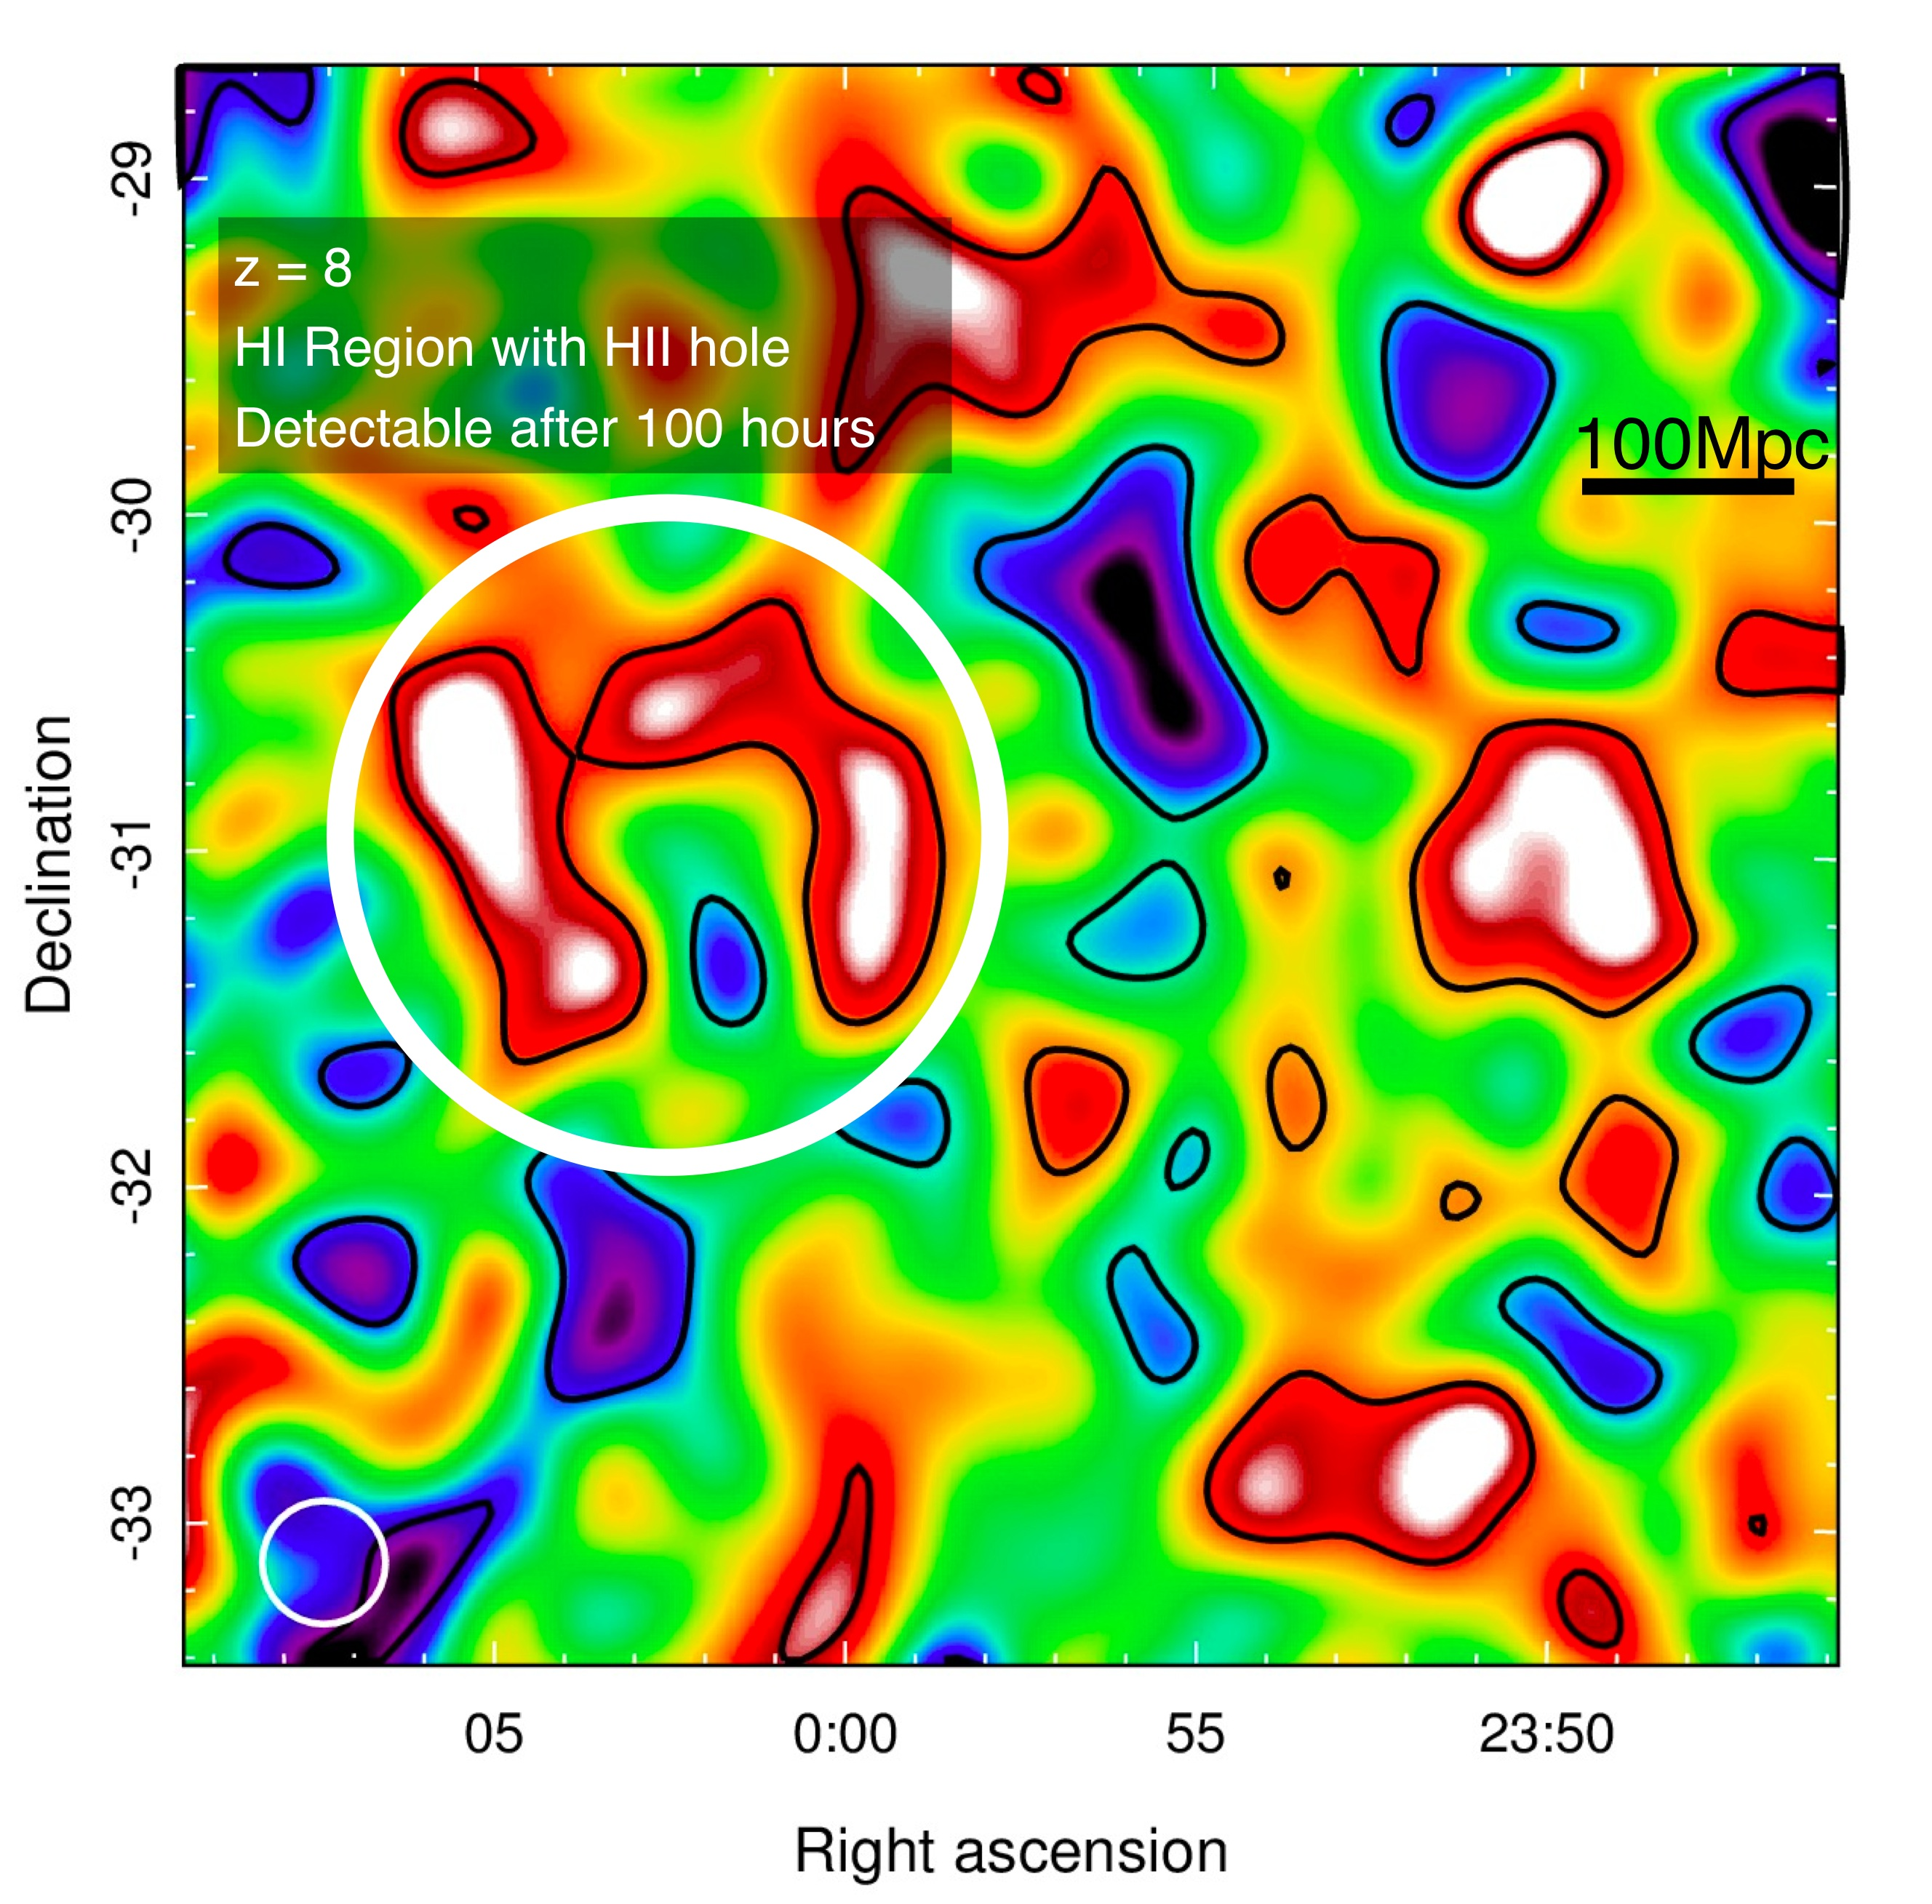
\includegraphics[height=2.5in]{plots/HERA_z8_SNR_annotated_v2.jpg}
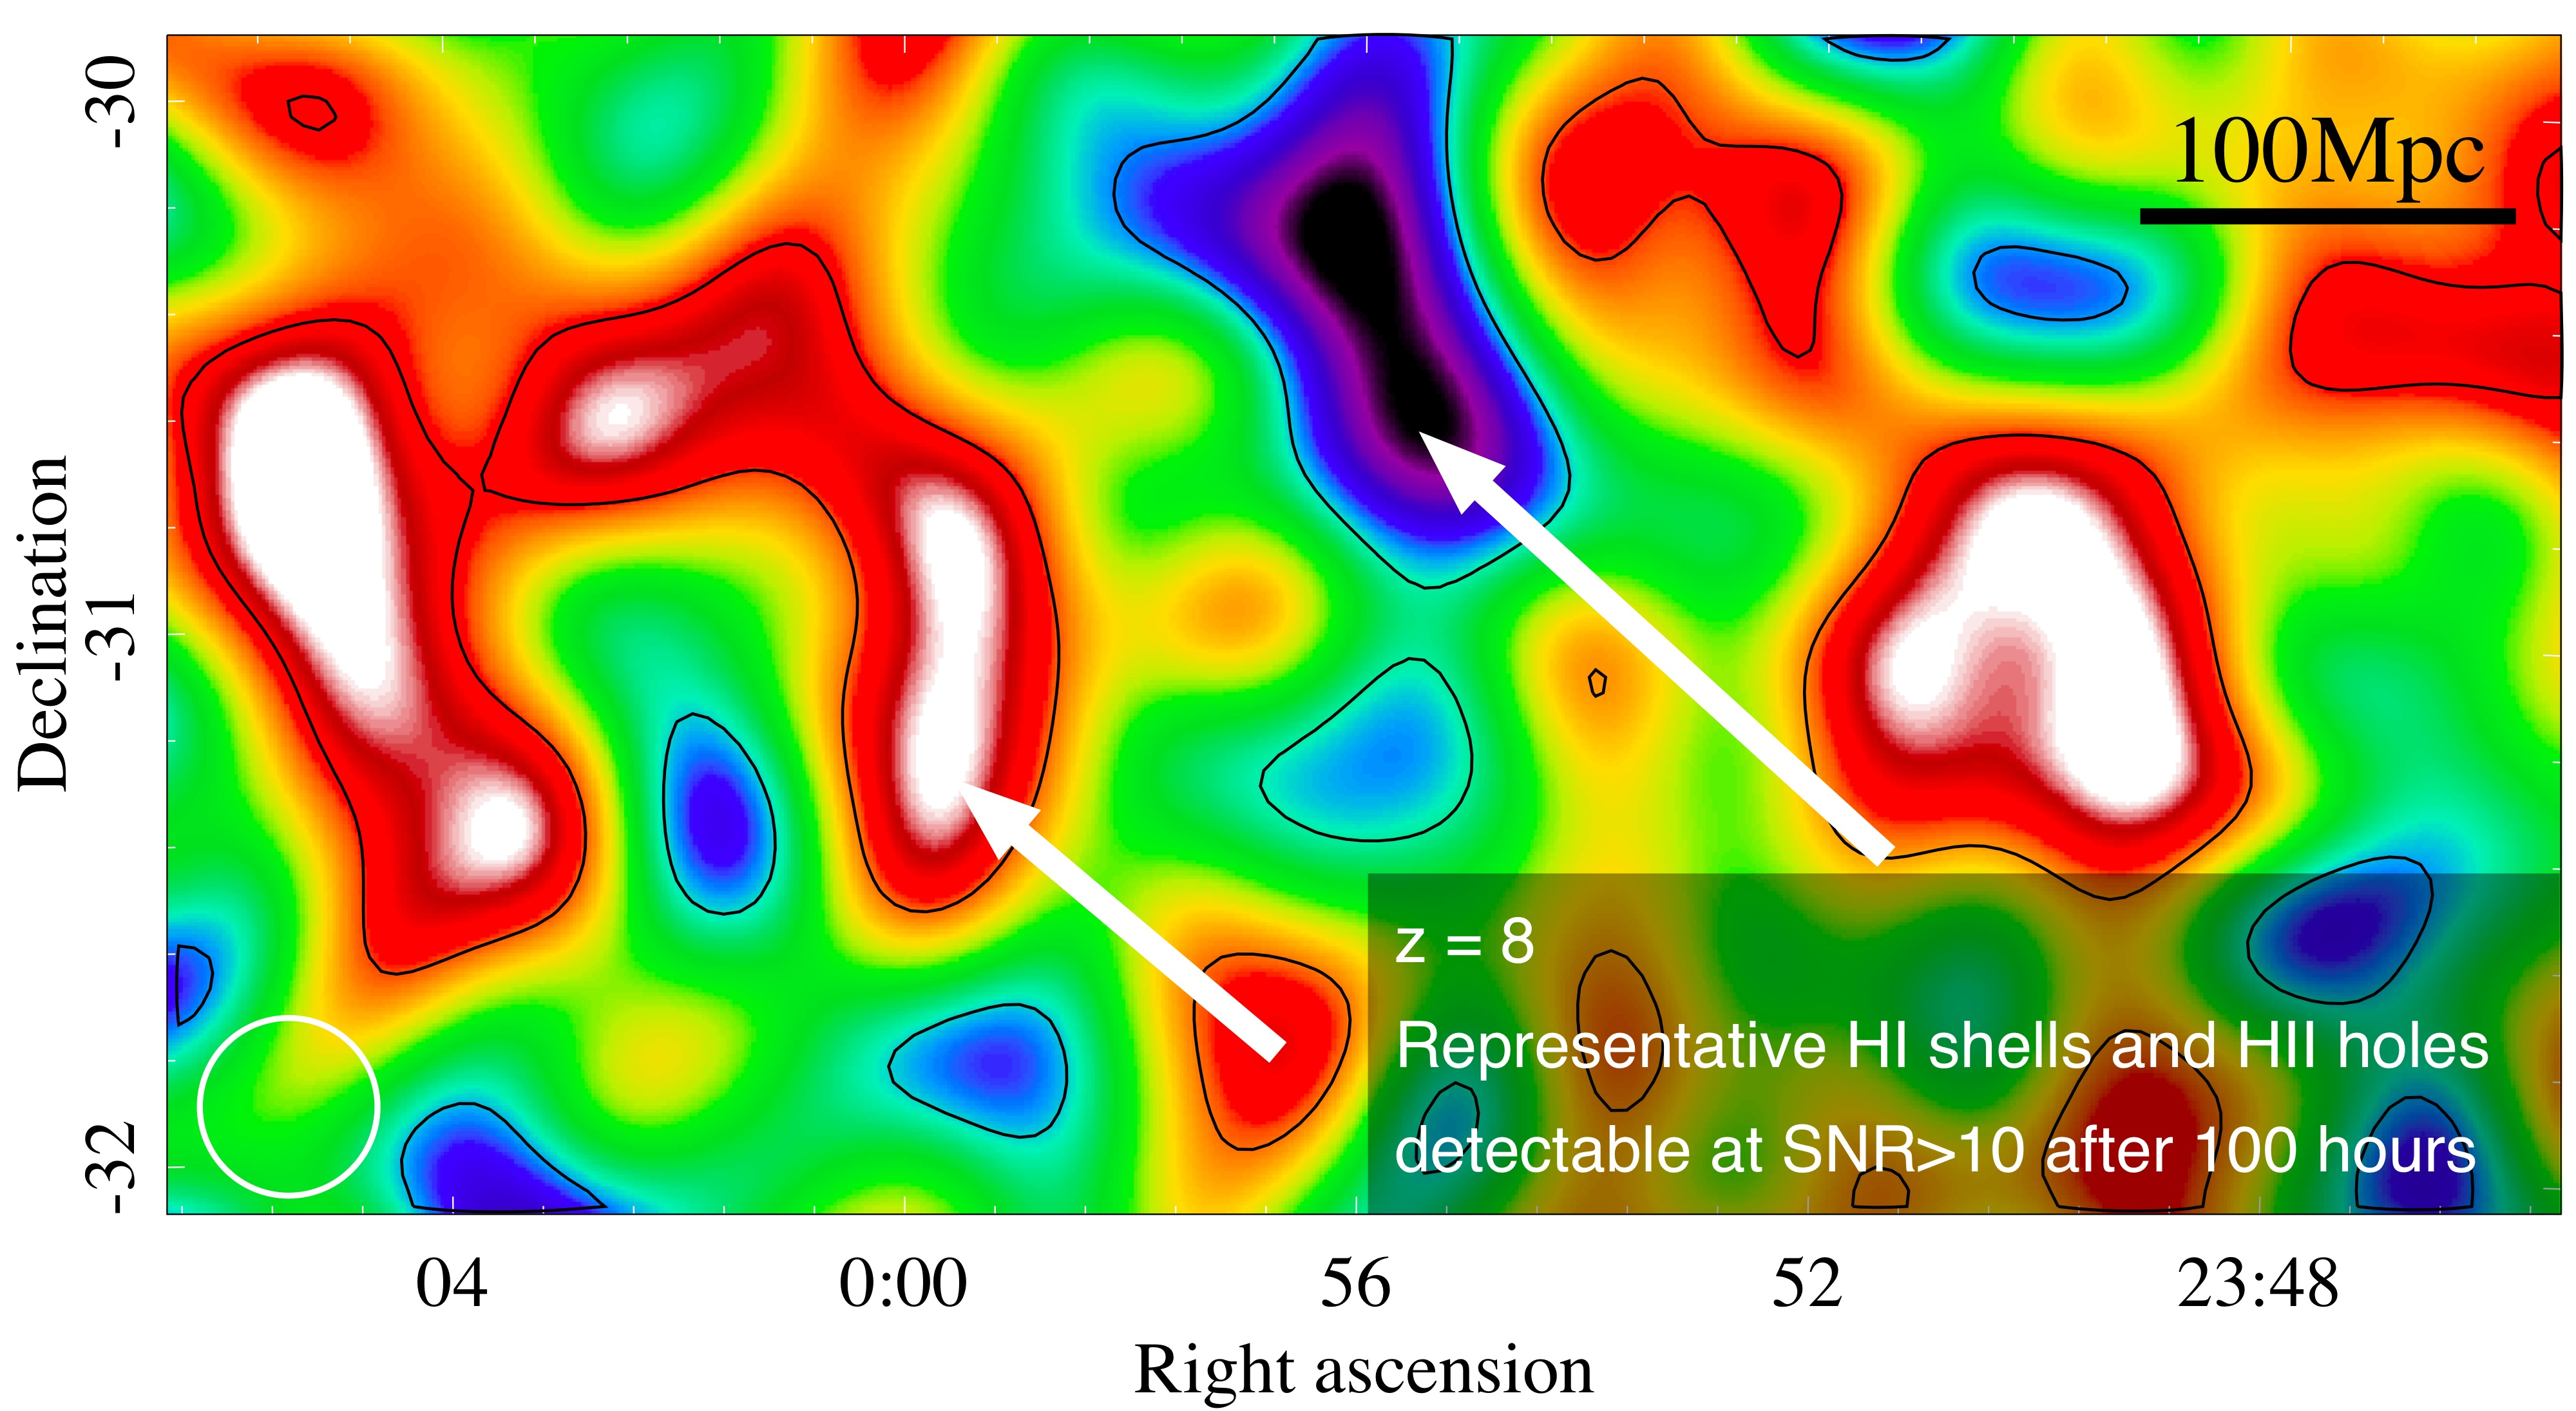
\includegraphics[height=2.5in]{plots/HERA_z8_SNR_wide_annotated.jpg}
% XXX waiting for version with "Characteristic HI shells and HII holes" in annotation
\caption{\small 
With a surface brightness sensitivity of 60~$\mu$Jy after filtering chromatic
foregrounds, HERA has the sensitivity
to directly image regions of neutral and ionized hydrogen.
Shown here is an instrumental simulation of reconstructed \HI emission at $z=8$,
assuming 100 hours of observing and 1~MHz of bandwidth with HERA~568.  The resulting
image has a resolution of 20\arcmin or about 50~cMpc; black contours
enclose regions detected at 10$\sigma$.
\label{imaging}}
\end{figure}

\vspace{-0.25in}
\section{Broader Impacts}
\label{BIsec}

An important part of the HERA program is training new
instrumentalists.  The project plan involves graduate students in all
stages of HERA development and observation. We will also fund an
undergraduate specialist position
at UC Berkeley's RAL, offered annually, with the goal of
mentoring the individual in the skills required to pursue graduate
research in instrumentation.

A second important activity of the HERA program is the diversity
efforts that naturally afford themselves working in Africa. PAPER has
an admirable history of enlisting interns from South African
Universities as part of major engineering deployments, with the work
applied as practical training within their academic program.
For HERA, we are establishing formal collaborations with South African
faculty, to engage doctoral students from these institutions in HERA,
including working visits between students in both directions. We will
recruit talented South African undergraduate and masters students for
3-month internships at the HERA partner institutions. Each year, one
institution will host the SA student team, providing an REU-like
experience focused on helping commission and operate HERA. This
experience will familiarize the students with US graduate education,
and give them the research experience and professional contacts needed
to successfully apply for graduate education the USA, should they
choose to do so.

%Notes:
%
%1. For the final proposal, we should get a supporting letter from 
%Durban and other Unviersities wrt student program. 
%
%2. I have read the 'Faculty Bridges' documents from Sheth at NRAO.
%Unfortunately, this program is just getting started, and it is not
%formally recognized by the NSF, nor funded. If this becomes more
%concrete over the next 4 months, we might consider adding a sentence
%that student exchanges will be facilitated by the formal agreements
%established by the 'Faculty Bridges' program.  However, for now, I
%have left this out.

\vspace{5 pt}
\noindent {\bf Public Data Products.}
On the HERA timescale a number of new observations will come on line that would
benefit from cross-comparison with the power spectra and images produced by
HERA. These include providing the reionization environment for JWST and ALMA
galaxy and cluster observations; cross-correlation with WFIRST near-IR surveys;
and cross-correlation with CMB polarization observations. The HERA measurements
will be released to the community after an 18~month proprietary period and
hosted at MIT. These data products will include foreground subtracted cubes for
cross-correlation, deep images of reionization from HERA~568, compressed
visibilities for re-analysis, snapshot continuum images for transient
observations, and wide-field maps from the survey made in the first two years.
% XXX mcquinn: add cross-correlations with LSST, which will find z~6-8 galaxies, 30-m telescopes

% XXX include some of this above
%In parallel to the
%unique capabilities of the 21~cm line as a probe of neutral gas during
%reionization, powerful
%techniques are being explored to probe 
%the distribution of star forming galaxies and AGN droving reionization,
%and the ionized regions themselves.  
%CO and [CII] `intensity mapping' experiments \citep{carilli2011,lidz_et_al2011,gong_et_al2011}, 
%and wide-field
%near-IR galaxy surveys by WFIRST, are being designed to map the
%galaxy distributions during reionization.
%Follow-up high-resolution imaging of representative
%samples of these first galaxies with the JWST and ALMA will provide exquisite
%details of the distribution of the gas, dust, stars, and AGN inside the first
%galaxies. Likewise, there are signatures of large-scale structure in CMB images
%caused by streaming motions of ionized
%structures during reionization \citep{alvarez_et_al2006,tashiro_et_al2010}.
%
%Cross-correlating
%the 21~cm signal with these complementary views of reionization
%can potentially provide a complete imaging inventory of the sources and sinks of
%ionizing photons, and better constrain the physical processes involved in the
%formation of the first galaxies and AGN, and their influence on the neutral IGM
%(see \citealt{pritchard_loeb2012} for a review).  
%The cross correlation between 21~cm maps and very wide field galaxy distributions and the
%ionized gas distribution increases the reliability
%of each measurement,
%since foreground systematics are independent for the different
%techniques \citep{gong_et_al2011,alvarez_et_al2006,tashiro_et_al2010}. 
%The goal of imaging of
%reionization on 20' scales in year
%5 of HERA is well matched to the expected first results of intensity
%mapping experiments of large-scale structure in the galaxy distribution, as
%well as the final analysis of Planck CMB anisitropies. 
%We will work with teams from the complementary
%reionization studies to optimize the cross correlation analyses, thereby
%enhancing scientific return on all experiments. 
%

% TBD:
%following could be throw-away/repeditive: 
%
%The combination of imaging of the neutral IGM from the 21~cm experiments, with large scale galaxy distributions from CO/[CII] intensity mapping experiments and WFIRST surveys, and imaging of large scale ionized structures through CMB experiments, will map-out the full three dimensional structure of the Universe during reionization. In parallel, ALMA and JWST will probe the details of individual galaxies during reionization. Together, these programs will fulfill one of the primary Discovery objectives of NWNH, namely, exploring cosmic dawn and the epoch of first galaxy formation.
%
%1. A. Liu and M. Tegmark. PRD, 83:103006, 2011.
%2. C. L. Carilli, ApJ, 730:L30, 2011.
%3. A. Lidz et al. ApJ, 741:70, 2011.
%4. Y. Gong et al. ApJ, 728:L46, February 2011.
%5. http://www.ipac.caltech.edu/wfirst/overview/science/surveys/
%6. Alvarez et al. 2006, ApJ 647, 840
%7. Tashiro et al. 2010, MNRAS 420, 2617
%
%
%notes:
%
%1. Maybe Steve F. can put in some more interesting detailed physical implications?
%
%2. James can fill-in some CMB pol cross correlation details
%
%2. perhaps include fig 18 from Pritchard and Loeb (from Lidz et al., I think), or maybe one of the cross correlation PS analyses?

\vspace{-0.25in}
\section{Project Management Plan}
\label{PMPsec}

This project balances the light-weight management structure of current PAPER/MWA
activities and the more formal structure required for larger-scale projects.
Construction management is centered at UC Berkeley's Radio Astronomy Laboratory
(RAL), headed by Parsons as the Project Director and DeBoer as
Project Manager. They will be assisted by Bob Goeke at MIT as a part-time
Project Engineer with a particular emphasis on interfacing with the US-based
antenna contractor.  A Site Manager will split their time between South Africa
and Berkeley and manage the construction activities by local South African
contractors. A SKA-SA Liaison will coordinate HERA, Meerkat, and SKA site
activities (supported by SKA-SA). Governance will be provided by an Executive Board comprising
this proposal's senior investigators, and will be operate using
super-majority policies. 

The scientific capability of HERA and the data analysis and publication will be
overseen by the Science Panel, and chaired by the Project Scientist, Bowman. These
positions will rotate as needed expertise changes, and are appointed by the
Executive Board.  As with the MWA and PAPER, observing
will be performed remotely with occasional site support
and maintenance headed by the Site Manager.

The estimated inherent contingency is $\sim$15\%, anticipating that additional project 
risk and contingency are handled by reducing
build-out with associated de-scoping of science capabilities.
A baseline design using
existing hardware establishes a low-risk path to core functionality and science.  Improved functionality
results from successful development activities or is otherwise de-scoped.


\section{Why Now? Why Us?}

This HERA proposal follows the vision for 21~cm observations laid out in NWNH.
PAPER and the MWA have already succeeded in the primary task envisioned in
NWNH---characterizing the astrophysical foregrounds and developing the hardware
and analysis advances needed to suppress the contamination. The discovery and
characterization of the EoR Window and the development of precision foreground
mitigation techniques have shown that foregrounds can be suppressed to the current level
thermal noise (\S \ref{LessonsSec}; \citealt{parsons_et_al2013}). While the MWA
and PAPER are pushing hard to detect the EoR power spectrum, %budget constraints have
%dictated that 
a marginal detection is the best these instruments can achieve.
HERA will both ensure a high significance detection of the \HI 21~cm signal, as
well as provide powerful constraints on the rise and fall of reionization, how
early stars and structure formed, and physical processes at the end of the
cosmic dark ages (Figures \ref{fig:x_i_Xray} \& \ref{fig:eor_pspec}).

As envisioned in NWNH, the US EoR projects (PAPER, MWA, EDGES, MITEoR) have
pooled their expertise to develop the second generation HERA observatory. This
has created a small collaborative team with a deep well of scientific
experience---the majority of papers on EoR observations are authored by members
of the HERA team. By leveraging this expertise, the HERA design is significantly
less expensive than envisioned in NWNH, while having greater scientific reach.

The last few years have been very productive for the EoR community---we
understand the foreground contamination and we are pushing the current
instruments to their thermal limits. We are now ready to build the HERA
instrument envisioned in NWNH and realize the scientific promise of 21~cm
cosmology.
Studying the formation of the first luminous structures after the Big
Bang and how they reionize the Universe is a primary driver for all % XXX check on "all"
major astronomical facilities over the next decade (ref: NWNH).
Such studies will include direct observation of the stars, gas, dust, and AGN in the
first galaxies using the JWST, LSST, TMT, ALMA, CCAT, and the JVLA. HERA is % XXX is it ok to mention CCAT?
a unique and necessary element in this panchromatic arsenal, providing
the large scale context in which the complex process of first galaxy
formation plays out.

\clearpage
\setcounter{page}{1}
\thispagestyle{empty}
%\bibliographystyle{apj}
%\bibliographystyle{hapj}
\bibliographystyle{jponew}
%\bibliographystyle{unsrt}
\bibliography{biblio}


\end{document}

